\documentclass{homework}
\newcommand{\R}{\textbf{R}}
\newcommand{\dee}{\;\text{d}}
\newcommand{\eps}{\varepsilon}
\newcommand{\pl}[2]{\frac{\partial #1}{\partial #2}}
\newcommand{\dl}[2]{\frac{\text{d} #1}{\text{d} #2}}
\newcommand{\sgn}{\text{sgn}}
\newcommand{\bigoh}{\mathcal{O}}
\usepackage{enumitem}

\newcommand{\hwclass}{Math 6108}
\newcommand{\hwname}{Jacob Hauck}
\newcommand{\hwtype}{Homework}


\usepackage{listings}
\usepackage{booktabs}

\newcommand{\hwnum}{5 and 6}
\renewcommand{\questiontype}{Problem}

\begin{document}
	\maketitle
	
	\question
	Consider the IVP
	\begin{gather*}
		y'' + x^2y = (x^2-4)\sin(2x), \qquad x > 0 \\
		y(0) = 0, \quad y'(0) = 2.
	\end{gather*}
	In order to solve this IVP numerically, we rewrite it as a system of ODEs by defining $z = y'$. Then we can equivalently solve
	\begin{align*}
		y' &= z \\
		z' &= -x^2y + (x^2-4)\sin(2x) \\
		y(0) &= 0, \qquad z(0) = 2.
	\end{align*}
	For all numerical solutions, we approximation $y(x_n)$ and $z(x_n)$ by $y^n$ and $z^n$ at the points $\{x_n\}_{n=0}^N$, which are evenly spaced on $[0,1]$ by $k = \frac{1}{N}$.
	
	\begin{alphaparts}
		\questionpart As the BDF2 method is a two-step method, we need to obtain $y^1$ and $z^1$ before we can start the main iteration. For this we can use the backward Euler method, which has second-order local truncation error to match the second-order global truncation error of the BDF2 method. This leads to the following implicit scheme
		\begin{align*}
			y^{n+1} &= \frac{1}{3}\left[4y^n - y^{n-1} + 2kz^{n+1}\right] && n =1,2,\dots, N-1\\
			z^{n+1} &= \frac{1}{3}\left[4z^n - z^{n-1} +2k(-x_{n+1}^2y^{n+1} + (x_{n+1}^2 - 4)\sin(2x_{n+1}))\right]&& n=1,2,\dots,N-1 \\
			y^1 &= y^0 + kz^1 \\
			z^1 &= z^0 + k(-x_1^2y^1 + (x_1^2 -4)\sin(2x_1)) \\
			y^0 &= 0 \\
			z^0 &= 2.
		\end{align*}
		Since the original equation is linear, we can easily solve the implicit equations above to obtain the following equivalent, explicit scheme
		\begin{align*}
			z^{n+1} &= \frac{\frac{1}{3}\left[4z^n - z^{n-1} + 2k\left[-\frac{1}{3}x_{n+1}^2(4y^n - y^{n-1}) + (x_{n+1}^2 - 4)\sin(2x_{n+1})\right]\right]}{1 + \frac{4k^2}{9}x_{n+1}^2} && n = 1,2,\dots,N-1\\
			y^{n+1} &= \frac{1}{3}\left[4y^n - y^{n-1} + 2kz^{n+1}\right] && n =1,2,\dots, N-1\\
			z^1 &= \frac{z^0 + k(-x_1^2y^0 + (x_1^2-4)\sin(2x_1))}{1 + k^2x_1^2} \\
			y^1 &= y^0 + kz^1 \\
			y^0 &= 0 \\
			z^0 &= 2.
		\end{align*}
		
		\questionpart In Table \ref{tab:p1b} are the errors and convergences rates of the method from part (a). The table shows that the method empirically has convergence rate of 2, as expected theoretically.
		
		\begin{table}[h]
			\centering
			\begin{tabular}{@{}lll@{}}
				\toprule
				$h$ & Error & Rate \\
				\midrule
				1/8 & 8.457332e-02 & - \\
				1/16 & 2.133647e-02 & 1.986881 \\
				1/32 & 5.319670e-03 & 2.003913 \\
				1/64 & 1.325627e-03 & 2.004662 \\
				1/128 & 3.307156e-04 & 2.003012 \\
				1/256 & 8.258288e-05 & 2.001677 \\
				\bottomrule
			\end{tabular}
			\caption{Errors at $t=1$ with convergence rates using the BDF2 method in (a)}
			\label{tab:p1b}
		\end{table}
		
		\questionpart Since the TR-BDF2 method is a one-step method, we can apply the method immediately to obtain the following implicit scheme
		\begin{align*}
			y_*^{n+1} &= y^n + \frac{k}{4}\left[z^n + z_*^{n+1}\right] \\
			z_*^{n+1} &= z^n + \frac{k}{4}\left[-x_n^2y^n + (x_n^2 - 4)\sin(2x_n) - x_{n+1/2}^2y_*^{n+1} + (x_{n+1/2}^2-4)\sin(2x_{n+1/2})\right] \\
			y^{n+1} &= \frac{1}{3}\left[4y_*^{n+1} - y^n + kz^{n+1}\right] \\
			z^{n+1} &= \frac{1}{3}\left[4z_*^{n+1} - z^n + k\left[-x_{n+1}^2y^{n+1} + (x_{n+1}^2 - 4)\sin(2x_{n+1})\right]\right] \\
			&\text{for $n = 0, 1, \dots, N-1$, and} \\
			y^0 &= 0 \\
			z^0 &= 2,
		\end{align*}
		where $x_{n+1/2} = x_n + \frac{k}{2}$. As in part (a), we can solve this scheme to obtain an equivalent explicit scheme
		\begin{align*}
			z_*^{n+1} &= \frac{z^n + \frac{k}{4}\left[-x_n^2y^n + (x_n^2-4)\sin(2x_n) -x_{n+1/2}^2\left(y^n + \frac{k}{4}z^n\right) + (x_{n+1/2}^2-4)\sin(2x_{n+1/2})\right]}{1 + \frac{k^2}{16}x_{n+1/2}^2} \\
			y_*^{n+1} &= y^n + \frac{k}{4}\left[z^n + z_*^{n+1}\right] \\
			z^{n+1} &= \frac{\frac{1}{3}\left[4z_*^{n+1} - z^n + k\left[-\frac{x_{n+1}^2}{3}\left[4y_*^{n+1} - y^n\right] + (x_{n+1}^2 -4)\sin(2x_{n+1})\right]\right]}{1+\frac{k^2}{9}x_{n+1}^2} \\
			y^{n+1} &= \frac{1}{3}\left[4y_*^{n+1} - y^n + kz^{n+1}\right]\\
			&\text{for $n = 0,1,\dots,N-1$, and} \\
			y^0 &= 0 \\
			z^0 &= 2.
		\end{align*}
		
		\questionpart In Table \ref{tab:p1d} are the errors and convergences rates of the method from part (c). The table shows that the method empirically has convergence rate of 2, as expected theoretically.
		
		\begin{table}[h]
			\centering
			\begin{tabular}{@{}lll@{}}
				\toprule
				$h$ & Error & Rate \\
				\midrule
				1/8 & 5.161865e-04 & -\\
				1/16 & 1.369409e-04 & 1.914339\\
				1/32 & 3.531733e-05 & 1.955105\\
				1/64 & 8.970516e-06 & 1.977114\\
				1/128 & 2.260645e-06 & 1.988456\\
				1/256 & 5.674363e-07 & 1.994204\\
				\bottomrule
			\end{tabular}
			\caption{Errors at $t=1$ with convergence rates using the TR-BDF2 method in (c)}
			\label{tab:p1d}
		\end{table}

	\end{alphaparts}
	
	\question Consider the BVP
	\begin{gather*}
		y'' + x^2y = (x^2-4)\sin(2x), \qquad 0 < x < \pi \\
		y(0) = 0, \qquad y'(\pi) + 2y(\pi) = 2.
	\end{gather*}
	For all numerical solutions, we approximation $y(x_n)$ by $y_n$ at the points $\{x_n\}_{n=0}^N$, which are evenly spaced on $[0,1]$ by $h = \frac{1}{N}$.
	\begin{alphaparts}
		\questionpart Using the centered difference method to approximate $y''$ on the interior of the domain, we get the following scheme for the interior points $y_1, y_2, \dots y_{N-1}$
		\begin{equation*}
			\frac{y_{n+1} - 2y_n + y_{n-1}}{h^2} + x_n^2y_n = (x_n^2- 4)\sin(2x_n), \qquad n = 1, 2, \dots, N-1.
		\end{equation*}
		The left boundary condition gives the discrete condition $y_0 = 0$, but the right boundary condition involves the first order derivative $y'$; to approximate this with a centered difference, we would need a point $x_{N+1} = x_N + h$ outside of the domain (assuming that $y'$ can be continuously extended, giving us the approximation $y_{N+1} \approx y(x_{N+1})$). By enforcing the differential equation at the point $x_N$, we can obtain another equation involving the point $x_{N+1}$, which we can combine with the boundary condition to eliminate the need for information at $x_{N+1}$, as follows:
		\begin{gather*}
			\frac{y_{N+1}-y_{N-1}}{2h} + 2y_N = 2 \qquad \text{(right boundary condition)}\\
			\frac{y_{N+1} - 2y_N + y_{N-1}}{h^2} + x_N^2y_N = (x_N^2-4)\sin(2x_N) \qquad \text{(equation at $x_N$)}
		\end{gather*}
		Eliminating $y_{N+1}$ gives
		\begin{equation*}
			\frac{2y_{N} -2y_{N-1} +h^2\left[-x_N^2y_N + (x_N^2 - 4)\sin(2x_N)\right]}{2h} + 2y_N = 2.
		\end{equation*}
		Substituting the explicit condition $y_0 = 0$ into the $n =1$ equation and collecting all our equations together, we obtain the scheme
		\begin{align*}
			\left(x_1^2 - \frac{2}{h^2}\right)y_1 + \frac{1}{h^2}y_2 &= (x_1^2-4)\sin(2x_1) \\
			\frac{1}{h^2}y_{n-1} + \left(x_n^2 - \frac{2}{h^2}\right)y_n + \frac{1}{h^2}y_{n+1} &= (x_n^2-4)\sin(2x_n), \qquad n = 2,3,\dots, N-1 \\
			 -\frac{1}{h}y_{N-1} + \left(\frac{1}{h} -\frac{hx_N^2}{2} + 2\right)y_N &= 2-\frac{h}{2}(x_N^2-4)\sin(2x_N).
		\end{align*}
		We can write this system of equations in matrix-vector form $Ay = b$, where
		\begin{equation*}
			A = \left[\begin{matrix}
				x_1^2-\frac{2}{h^2} & \frac{1}{h^2} &  &  & & \\
				\frac{1}{h^2} & x_2^2 - \frac{2}{h^2} & \frac{1}{h^2} &  &  & \\
				 & \frac{1}{h^2} & x_3^3 - \frac{2}{h^2} & \frac{1}{h^2} & &\\
			     & & \ddots &  & \\
				 &  & \frac{1}{h^2} & x_{N-1}^2 - \frac{2}{h^2} & \frac{1}{h^2} \\
				 &  &  & -\frac{1}{h} & \frac{1}{h} - \frac{hx_N^2}{2} +2
			\end{matrix}\right],
		\end{equation*}
		where empty entries are assumed to be 0, and
		\begin{equation*}
			y = \left[\begin{matrix}y_1 \\ y_2 \\ \vdots \\ y_N\end{matrix}\right], \qquad b = \left[\begin{matrix}(x_1^2 - 4)\sin(2x_1) \\[0.3em] (x_2^2-4)\sin(2x_2) \\ \vdots \\ (x_{N-1}^2-4)\sin(2x_{N-1}) \\[0.3em] 2 - \frac{h}{2}(x_N^2 - 4)\sin(2x_N)\end{matrix}\right].
		\end{equation*}
		
		\questionpart In Table \ref{tab:p2b} are the $\ell^2$ and $\ell^\infty$ errors of the scheme in part (a). Based on the table, the $\ell^\infty$ convergence rate is 2, and the $\ell^2$ convergence rate is 1.5, which is not surprising given the equivalence of the $\ell^2$ and $\ell^\infty$ norms:
		\begin{equation*}
			\lVert u \rVert_{\ell^\infty} \le \lVert u \rVert_{\ell^2} \le \sqrt{N}\lVert u \rVert_{\ell^\infty} \qquad \text{for all $u \in \R^N$.}
		\end{equation*}
		Indeed, let $e \in \R^{N+1}$ be a vector of errors defined by $e_n = |y_n - y(x_n)|$. If $\lVert e\rVert_{\ell^\infty} \approx h^2$, then the right inequality implies that $\lVert e \rVert_{\ell^2} \lesssim \left(\sqrt{N+1}\right)h^2 \approx h^{1.5}$ because $N \approx h^{-1}$.
		
		\begin{table}[h]
			\centering
			\begin{tabular}{@{}lllll@{}}
				\toprule
				$h$ & $\ell^2$ error & $\ell^2$ rate & $\ell^\infty$ error & $\ell^\infty$ rate \\
				\midrule
				$\pi$/8 & 2.219190e-01 & - & 1.280149e-01 & -\\
				$\pi$/16 & 6.790030e-02 & 1.708543 & 2.905806e-02 & 2.139301\\
				$\pi$/32 & 2.293204e-02 & 1.566053 & 6.987220e-03 & 2.056148\\
				$\pi$/64 & 7.996325e-03 & 1.519956 & 1.727129e-03 & 2.016342\\
				$\pi$/128 & 2.815873e-03 & 1.505755 & 4.305031e-04 & 2.004281\\
				$\pi$/256 & 9.943666e-04 & 1.501732 & 1.075450e-04 & 2.001083\\
				\bottomrule
			\end{tabular}
			\caption{Centered difference -- $\ell^2$ and $\ell^\infty$ errors with convergence rates}
			\label{tab:p2b}
		\end{table}
		
		\questionpart Using the centered difference method to approximate $y''$ on the interior of the domain, we get the following scheme for the interior points $y_1, y_2, \dots y_{N-1}$
		\begin{equation*}
			\frac{y_{n+1} - 2y_n + y_{n-1}}{h^2} + x_n^2y_n = (x_n^2- 4)\sin(2x_n), \qquad n = 1, 2, \dots, N-1.
		\end{equation*}
		The left boundary condition gives the discrete condition $y_0 = 0$, but the right boundary condition involves the first order derivative $y'$; to approximate this with a second-order, one-sided method, we recall from class that, for a function $u(t)$,
		\begin{equation*}
			u'(t) = \frac{-3u(t) + 4u(t+k) - u(t+2k)}{2k} + \bigoh(h^2).
		\end{equation*}
		Taking $u = y$, $k = -h$, and $t=\pi$, this implies that
		\begin{equation*}
			y'(\pi) = \frac{3y(\pi) - 4y(\pi - h) + y(\pi - 2h)}{2h} + \bigoh(h^2).
		\end{equation*}
		This leads to the second-order, one-sided discretization of the right boundary condition
		\begin{equation*}
			\frac{3y_N - 4y_{N-1} + y_{N-2}}{2h} + 2y_N = 2.
		\end{equation*}
		Combining the left boundary condition with the first interior equation, we have the scheme
		\begin{align*}
			\left(x_1^2 -\frac{2}{h^2}\right)y_1 + \frac{1}{h^2}y_2 &= (x_1^2-4)\sin(2x_1) \\
			\frac{1}{h^2}y_{n-1} + \left(x_n^2 - \frac{2}{h^2}\right)y_n + \frac{1}{h^2}y_{n+1} &= (x_n^2- 4)\sin(2x_n), \qquad n = 2, 3, \dots, N-1 \\
			\frac{1}{2h}y_{N-2} - \frac{2}{h}y_{N-1} + \left(2 + \frac{3}{2h}\right)y_N &= 2.
		\end{align*}
		This system of equations can be written in matrix-vector form $Ay=b$, where
		\begin{equation*}
			A = \left[\begin{matrix}
				x_1^2 - \frac{2}{h^2} & \frac{1}{h^2} & & \\
				\frac{1}{h^2} & x_2^2 - \frac{2}{h^2} & \frac{1}{h^2} & \\
				& \frac{1}{h^2} & x_3^2 - \frac{2}{h^2} & \frac{1}{h^2} & \\
				& & \ddots & & \\
				& & \frac{1}{h^2} & x_{N-1}^2 - \frac{2}{h^2} & \frac{1}{h^2} \\[0.3em]
				& & \frac{1}{2h} & -\frac{2}{h} & 2 + \frac{3}{2h}
			\end{matrix}\right],
		\end{equation*}
		where blank entries are assumed to be 0, and
		\begin{equation*}
			y = \left[\begin{matrix}y_1 \\ y_2 \\ \vdots \\ y_N\end{matrix}\right], \qquad b = \left[\begin{matrix}
				(x_1^2-4)\sin(2x_1) \\ (x_2^2 - 4)\sin(2x_2) \\ \vdots \\ (x_{N-1}^2-4)\sin(2x_{N-1}) \\ 2
			\end{matrix}\right].
		\end{equation*}
		
		\questionpart
		In Table \ref{tab:p2d} are the $\ell^2$ and $\ell^\infty$ errors of the scheme in part (a). Based on the table, it seems that the $\ell^\infty$ convergence rate is 2, and the $\ell^2$ convergence rate is 1.5 (using a few smaller step sizes showed that this is really the case).
		
		\begin{table}[h]
			\centering
			\begin{tabular}{@{}lllll@{}}
				\toprule
				$h$ & $\ell^2$ error & $\ell^2$ rate & $\ell^\infty$ error & $\ell^\infty$ rate \\
				\midrule
				$\pi$/8 & 3.827128e+00 & - & 1.973108e+00 & -\\
				$\pi$/16 & 1.390236e+00 & 1.460932 & 5.126718e-01 & 1.944362\\
				$\pi$/32 & 6.531083e-01 & 1.089936 & 1.730366e-01 & 1.566958\\
				$\pi$/64 & 2.674238e-01 & 1.288195 & 5.028926e-02 & 1.782755\\
				$\pi$/128 & 9.931652e-02 & 1.429022 & 1.322982e-02 & 1.926457\\
				$\pi$/256 & 3.559417e-02 & 1.480393 & 3.355599e-03 & 1.979151\\
				\bottomrule
			\end{tabular}
			\caption{One-sided difference -- $\ell^2$ and $\ell^\infty$ errors with convergence rates}
			\label{tab:p2d}
		\end{table}
		
	\end{alphaparts}
	
	\question Consider the boundary-value problem
	\begin{align*}
		&\varepsilon y'' - x^2y' - y = 0, \qquad 0 < x < 1\\
		&y(0) = 1, \qquad y(1) = 1,
	\end{align*}
	where $\varepsilon > 0$.
	
	\begin{alphaparts}
		\questionpart We approximation $y(x_n)$ by $y_n$ at the points $\{x_n\}_{n=0}^N$, which are evenly spaced on $[0,1]$ by $h = \frac{1}{N}$. To handle the boundary conditions, we simply set $y_0 = 1$ and $y_N = 1$. At the interior points, we can use central difference approximations of the derivatives to obtain the equations
		\begin{equation*}
			\varepsilon\frac{y_{n+1} - 2y_n + y_{n-1}}{h^2} -x_n^2\frac{y_{n+1} - y_{n-1}}{2h} - y_n = 0, \qquad n = 1, 2, \dots, N-1.
		\end{equation*}
		Combining the boundary conditions with the first and last of these equations, we obtain the scheme
		\begin{align*}
			\left(\frac{\varepsilon}{h^2} - \frac{x_1^2}{2h}\right)y_{2} - \left(\frac{2\varepsilon}{h^2} + 1\right)y_1 &= -\left(\frac{\varepsilon}{h^2} + \frac{x_1^2}{2h}\right) \qquad \text{(left BC)}\\
			- \left(\frac{2\varepsilon}{h^2} + 1\right)y_{N-1} + \left(\frac{\varepsilon}{h^2} + \frac{x_{N-1}^2}{2h}\right)y_{N-2} &= -\left(\frac{\varepsilon}{h^2} - \frac{x_{N-1}^2}{2h}\right) \qquad \text{(right BC)}\\
			\left(\frac{\varepsilon}{h^2} - \frac{x_n^2}{2h}\right)y_{n+1} - \left(\frac{2\varepsilon}{h^2} + 1\right)y_n + \left(\frac{\varepsilon}{h^2} + \frac{x_n^2}{2h}\right)y_{n-1} &= 0, \qquad n = 2, 3, \dots, N-2.
		\end{align*}
		We can write these equations in matrix-vector form $Ay = b$, where
		\begin{equation*}
			A = \left[\begin{matrix}
				-\frac{2\varepsilon}{h^2} - 1 & \frac{\varepsilon}{h^2} - \frac{x_1^2}{2h} \\
				\frac{\varepsilon}{h^2} + \frac{x_2^2}{2h} & -\frac{2\varepsilon}{h^2} - 1 & \frac{\varepsilon}{h^2} - \frac{x_2^2}{2h} \\
				& \frac{\varepsilon}{h^2} + \frac{x_3^2}{2h} & -\frac{2\varepsilon}{h^2} - 1 & \frac{\varepsilon}{h^2} - \frac{x_3^2}{2h} \\
				& & \ddots\\
				& & \frac{\varepsilon}{h^2} + \frac{x_{N-2}^2}{2h} & -\frac{2\varepsilon}{h^2} - 1 & \frac{\varepsilon}{h^2} - \frac{x_{N-2}^2}{2h}\\
				& & & \frac{\varepsilon}{h^2} + \frac{x_{N-1}^2}{2h} & -\frac{2\varepsilon}{h^2} - 1
			\end{matrix}\right],
		\end{equation*}
		where blank entries are assumed to be 0, and
		\begin{equation*}
			y = \left[\begin{matrix}y_1 \\ y_2 \\ \vdots \\ y_{N-1}\end{matrix}\right], \qquad b = \left[\begin{matrix}-\left(\frac{\varepsilon}{h^2} + \frac{x_1^2}{2h}\right) \\ 0 \\ \vdots \\ 0 \\ -\left(\frac{\varepsilon}{h^2} - \frac{x_{N-1}^2}{2h}\right)\end{matrix}\right].
		\end{equation*}
		
		\questionpart In Figure \ref{fig:exact} is the ``exact'' solution for $\varepsilon = .05$ and $h = 1/2048$.
		
		\begin{figure}
			\centering
			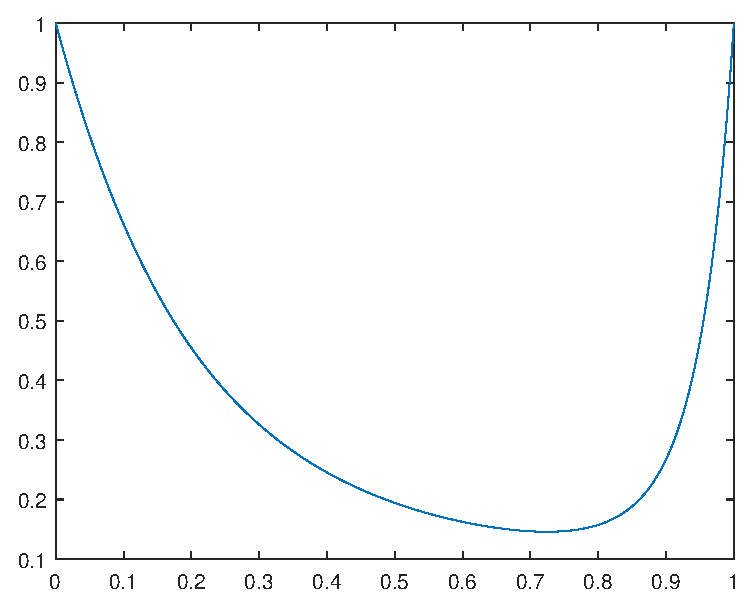
\includegraphics{p3_exact.eps}
			\caption{``Exact'' solution when $\varepsilon = 0.05$, computed using step size $h = 1/2048$}
			\label{fig:exact}
		\end{figure}
		
		\questionpart In Table \ref{tab:p3c} are the $\ell^2$ and $\ell^\infty$ errors (computed using the reference solution from (b)) with $\varepsilon = .05$. From the table, it appears that the centered difference method has a convergence rate of 2 in $\ell^\infty$ and 1.5 in $\ell^2$, just as it did on Problem 2.
		
		\begin{table}[h]
			\centering
			\begin{tabular}{@{}lllll@{}}
				\toprule
				$h$ & $\ell^2$ error & $\ell^2$ rate & $\ell^\infty$ error & $\ell^\infty$ rate \\
				\midrule
				1/8 & 8.952792e-02 & - & 8.748680e-02 & -\\
				1/16 & 3.516391e-02 & 1.348242 & 2.969501e-02 & 1.558845\\
				1/32 & 1.217098e-02 & 1.530651 & 6.755169e-03 & 2.136157\\
				1/64 & 4.237348e-03 & 1.522211 & 1.719463e-03 & 1.974034\\
				1/128 & 1.486917e-03 & 1.510838 & 4.260417e-04 & 2.012891\\
				1/256 & 5.188923e-04 & 1.518817 & 1.051005e-04 & 2.019226\\
				\bottomrule
			\end{tabular}
			\caption{Centered difference method with $\varepsilon = .05$ -- $\ell^2$ and $\ell^\infty$ errors with convergence rates}
			\label{tab:p3c}
		\end{table}
		
		\questionpart In Figure \ref{fig:p3d} is the ``exact'' solution for $\varepsilon = .05$ and $h = 1/2048$.
		
		\begin{figure}
			\centering
			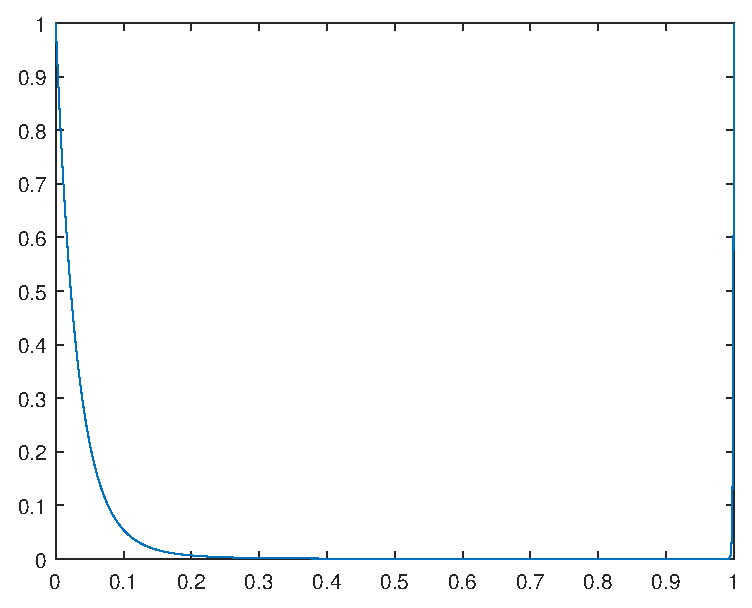
\includegraphics{p3d.eps}
			\caption{``Exact'' solution when $\varepsilon = 0.001$, computed using step size $h = 1/2048$}
			\label{fig:p3d}
		\end{figure}
		
		\questionpart In Table \ref{tab:p3e} are the $\ell^2$ and $\ell^\infty$ errors (computed using the reference solution from (b)) with $\varepsilon = .05$. From the table, it appears that the centered difference method has a convergence rate of 2 in $\ell^\infty$ and 1.5 in $\ell^2$, just as it did for $\varepsilon = 0.05$. The errors, however, are generally greater in this case than they were in the case of $\varepsilon = 0.05$, and the convergence rate doesn't settle down until the step size is already fairly small. This is likely due to the rapid change in the solution near $x =1$ when $\varepsilon$ is small (compare Figures \ref{fig:exact} and \ref{fig:p3d}, which show the $\varepsilon = 0.05$ and $\varepsilon = 0.001$ solutions).
		
		\begin{table}[h]
			\centering
			\begin{tabular}{@{}lllll@{}}
				\toprule
				$h$ & $\ell^2$ error & $\ell^2$ rate & $\ell^\infty$ error & $\ell^\infty$ rate \\
				\midrule
				1/8 & 8.839999e-01 & - & 7.051292e-01 & -\\
				1/16 & 8.168405e-01 & 0.113992 & 6.540523e-01 & 0.108482\\
				1/32 & 5.408442e-01 & 0.594841 & 4.827786e-01 & 0.438044\\
				1/64 & 2.517577e-01 & 1.103177 & 2.490745e-01 & 0.954784\\
				1/128 & 8.763561e-02 & 1.522447 & 8.247853e-02 & 1.594487\\
				1/256 & 2.856069e-02 & 1.617486 & 1.853421e-02 & 2.153828\\
				\bottomrule
			\end{tabular}
			\caption{Centered difference method with $\varepsilon = 0.005$ -- $\ell^2$ and $\ell^\infty$ errors with convergence rates}
			\label{tab:p3e}
		\end{table}
	
	\end{alphaparts}
\end{document}